\chapter{Datos}

\section{Obtención y análisis exploratorio de datos}

El dataset obtenido esta inicialmente constituido por 585001 tweets recolectados entre el 22 de mayo al 22 de junio del 2022, periodo dentro del cual ocurrieron la primera y la segunda vuelta de las elecciones presidenciales, el 29 de mayo y 19 de junio respectivamente. Para la extracción de los datos, se utilizaron 173 hashtags con contenido político que tuvieron lugar durante este periodo. este dataset fue filtrado para remover aquellos tweets que tuvieran menos de 5 palabras, aquellos que tuvieran una proporción de menciones,hashtags mayor al 20\% del total del texto, aquellos que tuvieran links o que provinieran de usuarios con un numero atípico de posteos. Esto redujo la base a 193348 tweets.  Los hashtags utilizados fueron etiquetados en uno de tres sectores políticos: Izquierda, Derecha y Neutro, dependiendo del contenido asociado a dichos hashtags y su tendencia política. En la tabla \ref{table:hashtags} se muestran los hashtags,así como su etiqueta política y cuantos tweets hubo para cada hashtags.

La distribución de los hashtags a través de los sectores políticos se puede evidenciar en el gráfico \ref{figure:tweets_cantidad_hashtags} donde se muestra que el sector neutro tiene mas de un  40\% del total de los hashtags, mientras que la izquierda y la derecha, tienen una cantidad semejante de aproximadamente un 28\%.


\begin{figure}[h]
	\caption{Porcentaje de Hashtags por sector político'}
	\centering
	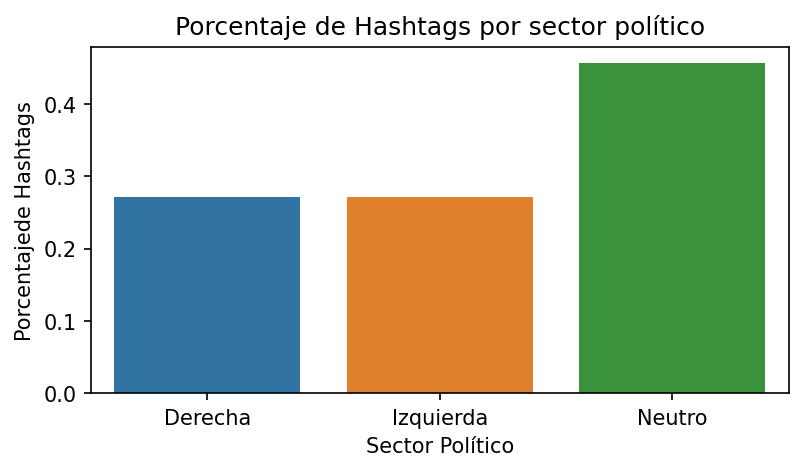
\includegraphics{../Images/EDA/Cantidad de Hashtags por sector politico.png} 
	\label{figure:tweets_cantidad_hashtags}
\end{figure}

De manera similar, el gráfico \ref{figure:tweets_porcentaje} muestra la distribución de tweets a lo largo de los sectores políticos. En este se aprecia que el sector neutro tiene la mayoría de los tweets, con mas del 46\%, luego se encuentra la izquierda con un 33\% y finalmente la derecha con cerca de un 29\%,



\begin{figure}[h]
	\caption{Porcentaje de tweets por sector político'}
	\centering
	\includegraphics{../Images/EDA/Porcentaje de tweets por sector político.png} 
	\label{figure:tweets_porcentaje}
\end{figure}


Al analizar la cantidad de tweets por sector a lo largo del tiempo, se obtienen los resultados observados en el gráfico \ref{figure:tweets_porcentaje_tiempo}, en donde se muestra que porcentaje del total de los tweets de cada sector, hubo en cada día. Se puede evidenciar que hubo algunas fechas particularmente importantes: el 24 de mayo que el dia de un debate y sobresale el sector neutro, el 29 de mayo que fue el dia de la primera vuelta y sobresalen los tres, el 9 de junio que fue el dia en el que salieron a la luz los llamados petro videos y sobresale la derecha y las fechas cercanas al 19 de junio que fue la fecha de la segunda vuelta y sobresalen los tres.

\begin{figure}[h]
	\caption{Porcentaje de tweets por sector político'}
	\centering
	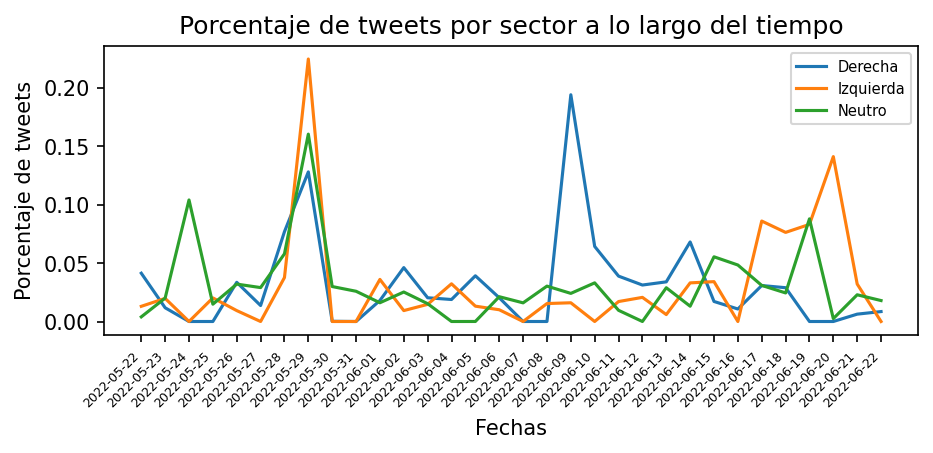
\includegraphics{../Images/EDA/Porcentaje de tweets por sector a lo largo del tiempo.png} 
	\label{figure:tweets_porcentaje_tiempo}
\end{figure}


\section{Etiquetado}

Para poder entrenar el modelo, se procedió a elaborar el etiquetado manual de una muestra del dataset. Esta muestra contiene 1200 tweets y se escogió de manera estratificada proporcional a la cantidad de tweets en los hashtags. La muestra fue etiquetada por el autor y los directores, quedando así 3 etiquetas independiente para cada uno de los tweets. Estos fueron etiquetados permitiendo múltiples etiquetas por tweets. Las etiquetas posibles fueron : Alegria, Agrado, Confianza, Admiración, Miedo, Incertidumbre, Sorpresa, Asombro, Tristeza, Decepción, Asco, Desagrado, Ira, Odio, Otra. Este etiquetado se llevo a cabo usando la plataforma web Label Studio. A partir de los resultados obtenidos, se obtuvo el grafico \ref{figure:correlacion_emociones}, en donde a partir de tener en cuenta las etiquetas de todos los etiquetadores se calcula la correlacion que tuvieron las distintas etiquetas. 

\begin{figure}[h]
	\caption{Correlación entre emociones'}
	\centering
	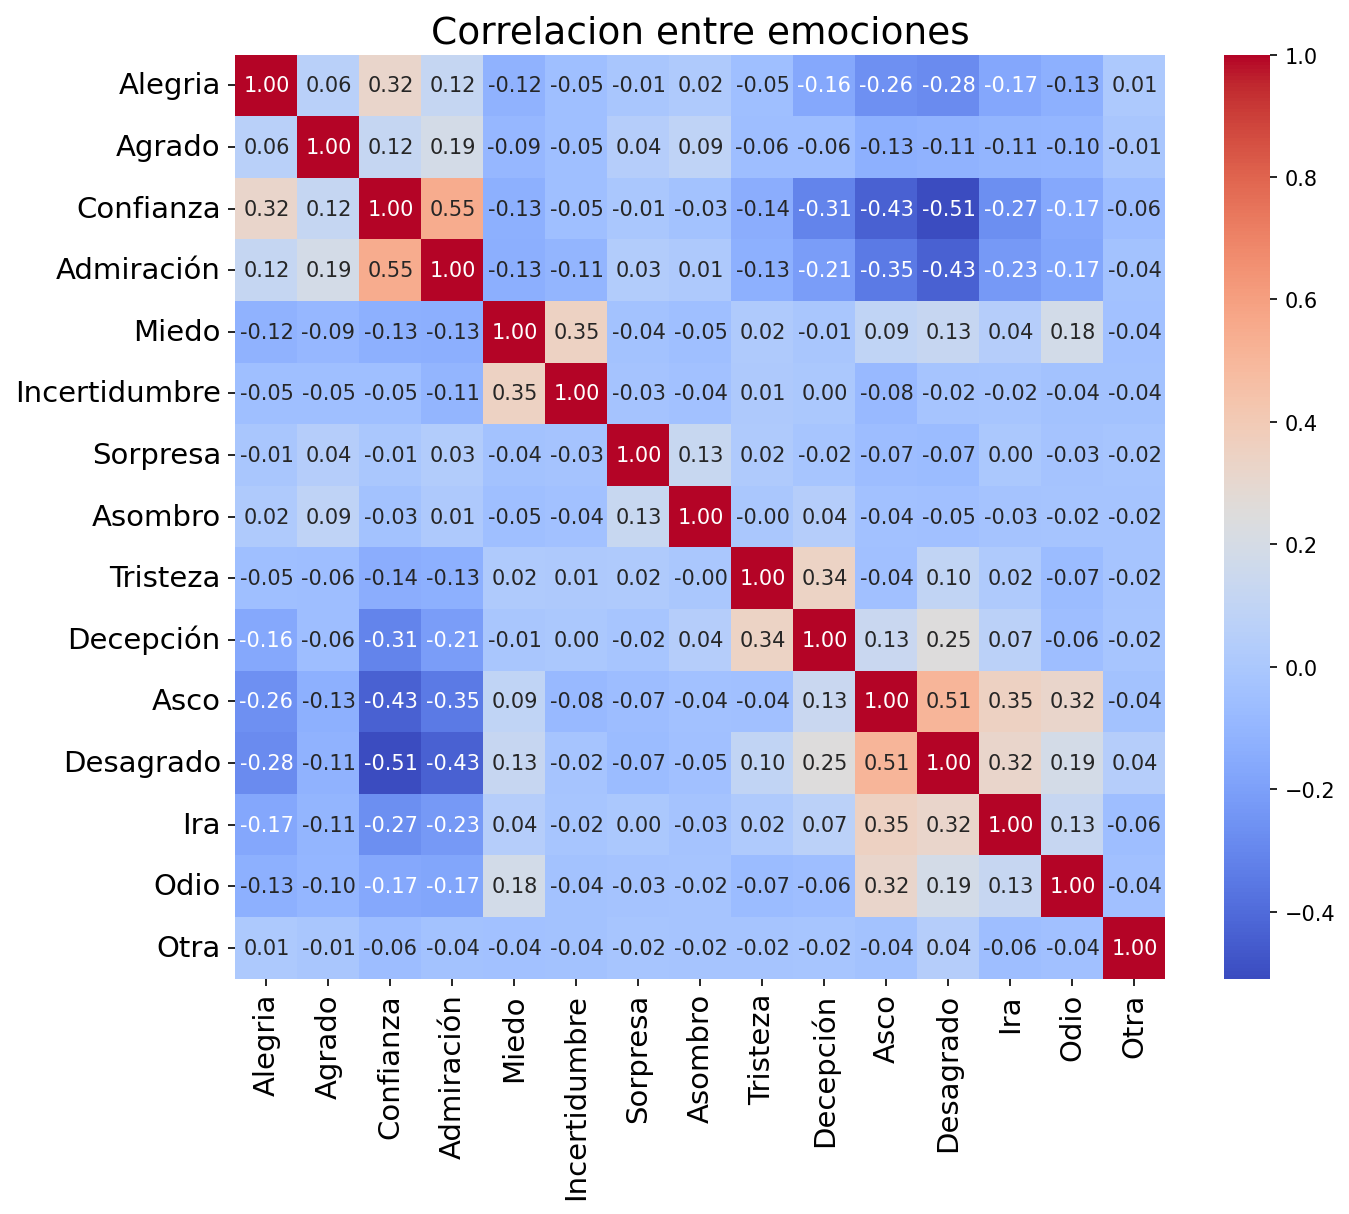
\includegraphics[scale=0.65]{../Images/EDA/emotions_correlations.png} 
	\label{figure:correlacion_emociones}
\end{figure}


A partir de estos resultados se construyeron 4 etiquetas agrupadoras, basado en cuan correlacionados estuvieron. Estas etiquetas fueron: Alegría que contiene las etiquetas Alegria, Agrado, Confianza y Admiración; Miedo que contiene las etiquetas Miedo e  Incertidumbre; Tristeza que contiene las etiquetas Tristeza y  Decepción; y 
Asco que contiene las etiquetas Asco, Desagrado, Ira y Odio. A cada tweet se le asigno una o varias de estas etiquetas finales si al menos dos de los etiquetadores asignaban alguna de las emociones que las componían a dicho tweet. Estas fueron las etiquetas con las que se entreno el modelo.

